
\section{Représentation et caractérisation des rhotiques et des sons \textg{simil-\textit{r}}} \label{sec:similr}


Le terme \textg{rhotique} fait appel à un concept en linguistique qui peut être habituellement représenté par le \textg{r} avec la lettre minuscule <r> ou majuscule <R> et leurs dérivés. 
Bien que le terme \textg{rhotique} semble être dérivé de la lettre grec <\begin{greek}ρ\end{greek}> \parencite{wieseRepresentationRhoticsRepresentation2011}, il semble que ce terme ait émergé à la fin des années 1960 (\autoref{fig:googlengramrhotic}) avec \href{http://phonetic-blog.blogspot.com/2010/07/rhotic.html}{John Wells} qui souhaitait parler de certains accents britanniques qui conservent le \textg{r} \parencite[78--79]{wellsJohnWellsPhonetic2010,wellsSoundsInteresting2014}.
Auparavant, l'expression \textg{\textit{r}-like sounds} était plutôt utilisée pour faire référence à ces sons représentés par le <r> et <R>, comme dans \textcite[78]{maddiesonPatternsSounds1984}. Nous traduirons \textg{\textit{r}-like sounds} par \textg{sons simil-\textit{r}}.
Les essais autour de la caractérisation du comportement des rhotiques et de ce qui en fait une classe phonologique ont donné une connotation de l'ordre de la phonologie au terme de rhotique. De son côté, le terme de son \textg{simil-r} est davantage resté dans une connotation de l'ordre de la phonétique.
Malgré la terminologie, le concept de rhotique reste d'ordinaire compris à travers les membres qui le composent, on parle alors de \textg{rhotiques}. Une première définition en extension consiste à décrire les différents segments appartenant à la catégorie des rhotiques. Le concept de rhotique subsiste par le besoin des linguistes de rendre compte de l'association qui existe entre les membres de la catégorie. Nous verrons, par la suite, la définition en intention utilisant le comportement phonologique des segments, qui doivent se comporter similairement.

\begin{figure}
	\centering
	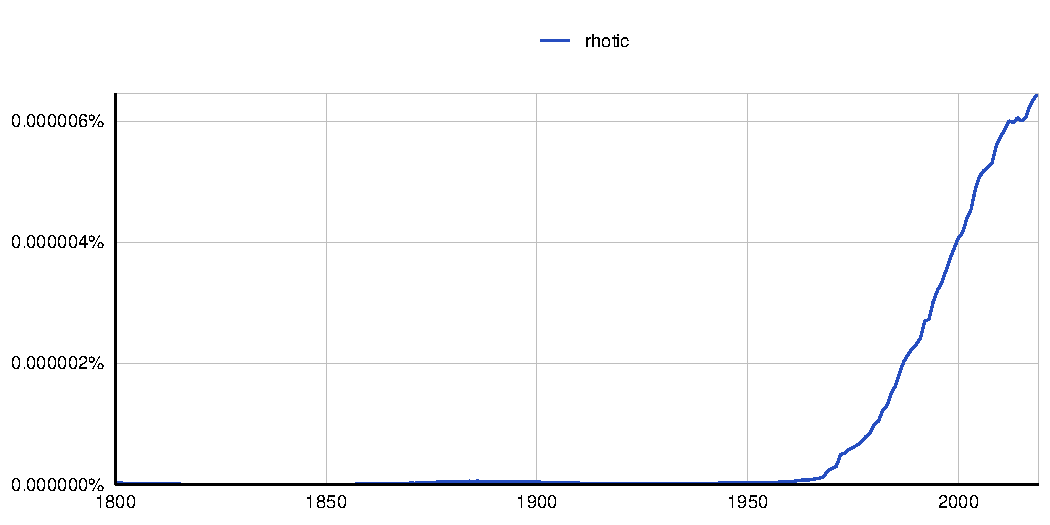
\includegraphics[width=1\linewidth]{images/google_ngram_rhotic}
	\caption[Google n-grams de \textg{rhotic}]{Fréquence de l'expression \textg{rhotic} à partir des données de Google Books en utilisant le package \texttt{ngramr} sur \texttt{RStudio} \parencite{rcoreteamLanguageEnvironmentStatistical2020}, à partir du jeu de données de Google 2019.}
	\label{fig:googlengramrhotic}
\end{figure}

\subsection{Les différents sons \textg{simil-\textit{r}}}

\textcite{wieseRepresentationRhoticsRepresentation2011} établit une liste de huit éléments sur la base des symboles de l'Alphabet Phonétique International qui leurs sont consacrés. Le  r est présent avec le ɾ, le ɹ, le ɺ ou encore le ɽ, le ɻ, le ʀ et le ʁ. Ces segments représentent le cœur des rhotiques et sont généralement présents dans les définitions en extension dans la littérature. À chaque symbole correspond un son et une description articulatoire (que nous appellerons aussi label descriptif dans cette thèse; \textcite{ladefogedSoundsWorldLanguages1996} parlent de définition du segment). \textcite{ladefogedSoundsWorldLanguages1996} dédient un chapitre de leur ouvrage sur les sons du monde aux rhotiques. Dès le début du chapitre, ils se réfèrent aux rhotiques comme une classe de sons comportant entre autres les mêmes huit symboles. On retrouve\footnote{Tous les segments dans la liste sont considérés comme voisés.} :

\begin{enumerate}
	\item Le trill alvéolaire (alveolar trill): r
	\item Le tap ou flap alvéolaire (alveolar tap or flap) : ɾ
	\item L'approximante alvéolaire (alveolar approximant) : ɹ
	\item Le flap alvéolaire latéral (alveolar lateral flap) : ɺ
	\item Le tap ou flap  rétroflexe (Retroflex tap or flap) : ɽ
	\item L'approximante rétroflexe (Retroflex approximant) : ɻ
	\item Le trill uvulaire (Uvular Trill) : ʀ
	\item La fricative uvulaire (Uvular Fricative) : ʁ
\end{enumerate}

Il est possible d'ajouter à ces segments des diacritiques pour spécifier d'autres articulations telles que {\fontspec{Charis SIL}◌̌  } pour les rhotiques fricatives (comme en tchèque), ou {\fontspec{Charis SIL}◌̞} pour les rhotiques approximantes (cf. \autoref{chap:soundcompa} pour un inventaire de diacritiques pouvant être retrouvés avec les rhotiques).\\ 

Nous décrivons brièvement les différents segments sur la base de \textcite{ladefogedSoundsWorldLanguages1996}. Il ne s'agit pas de faire une description complète des rhotiques mais de voir la diversité des articulations qui peuvent être mises en jeu. Le trill, le tap et le flap alvéolaire feront l'objet de sous-sections détaillées.

\subsubsection{Le trill alvéolaire}

Le trill alvéolaire est un son produit lorsque la pointe de la langue entre en vibration avec la crête alvéolaire en raison de conditions aérodynamiques, qui seront détaillées en \autoref{subsec:trill}. Ce trill alvéolaire (que nous appellerons simplement trill dans cette thèse) est représenté par le symbole API [r]. \textcite[218]{ladefogedSoundsWorldLanguages1996} mentionnent que les trills réalisés avec la pointe de la langue ont généralement deux ou trois périodes de vibration. Chaque période est constituée d'une phase ouverte et d'une phase fermée, pendant laquelle les articulateurs sont en contact.

\subsubsection{Les taps ou flaps alvéolaires et rétroflexes}

\textcite[231]{ladefogedSoundsWorldLanguages1996} établissent une distinction précise entre taps et flaps. Le flap implique un mouvement où la langue passe tangentiellement par la crête alvéolaire, alors que le tap implique un mouvement où la pointe de la langue se dirige vers la crête alvéolaire. La section sur les deux segments est relativement courte en comparaison à la présence relativement importante de ces segments dans les langues du monde comme allophones des rhotiques. Pour cela nous développerons d'autres études sur le tap et le flap en \autoref{subsec:acous_tap_flap} pour en comprendre les subtilités articulatoires et acoustiques.


\subsubsection{Les approximantes alvéolaires et rétroflexes}

La description de l'approximante alvéolaire a bénéficié des études portant sur la phonétique et la phonologie de l'anglais puisqu'il s'agit de la rhotique qu'on retrouve en anglais britannique du sud et en anglais états-unien. \textcite{ladefogedPreliminariesLinguisticPhonetics1971} mentionne que l'articulation de l'approximante anglaise peut être alvéolaire ou post-alvéolaire. La pointe de la langue se situe au niveau ou derrière la crête alvéolaire.
En utilisant Uldall (1958)\footnote{Uldall, Elizabeth. 1958. \textg{American \textg{molar} R and \textg{flapped} T.} \textit{Revista do Laboratorio de Fonetica Experimental, Universidad de Coimbra} 4: 103-6.} comme référence, \textcite[234]{ladefogedSoundsWorldLanguages1996} mentionnent qu'il existe aussi une articulation plus complexe, le \textg{bunched r} impliquant deux constrictions : une au niveau du pharynx bas et une au niveau du centre du palais. De plus, cette articulation ne s'accompagne pas d'une élévation de la pointe ou de la lame de la langue. Plusieurs articulations existent pour l'approximante de l'anglais américain bien qu'acoustiquement les segments issus de ces différentes articulations soient similaires.

\subsubsection{Le trill et la fricative uvulaire}

Comme le trill alvéolaire, le trill uvulaire est produit lorsque l'uvule rentre en vibration. 
En se basant sur les travaux de \textcite{delattrePharyngealFeaturesConsonants1971}, \textcite{ladefogedSoundsWorldLanguages1996}, montrent que, de la même manière que les trills alvéolaires, les trills uvulaires varient. Sur la base des travaux de \citeauthor{lindauStory1985}, ils mentionnent que les trills uvulaires intervocaliques sont plus longs que les alvéolaires (p. 226).
Ce son se retrouve en alternance avec la fricative uvulaire, qui est produite lors d'un rapprochement des articulateurs au niveau de la zone uvulaire entraînant de la friction mais sans vibration de l'uvule. Ce son est présent en français \parencite{lancasterBeginningsFrenchUvular1934,hambyePrononciationFrancaisContemporain2005,prematRouleFrancaisDans2018}, en allemand, en néerlandais \parencite{sebregtsSociophoneticsPhonologyDutch2014} et a fait l'objet de recherches en articulation et en acoustique \parencite{gendrotArticulatoryAcousticRealization2016}.

\subsection{Distribution des rhotiques}

Les différents segments n'ont pas la même distribution dans les langues du monde, certains sons étant plus fréquents que d'autres. Avec les données de UPSID, \textcite{maddiesonPatternsSounds1984} montre que, dans son échantillon, plus de 70\% des langues ont au moins une rhotique. Parmi les langues qui ont une rhotique, le trill est présent dans 47,5\% des cas, suivi du tap/flap dans 38,3\% des cas. Les fricatives et approximantes ne représentent que 13,5\%. Cet échantillon de langues permet à \citeauthor{maddiesonPatternsSounds1984} d'affirmer que les sons \textg{simil-\textit{r}} sont généralement voisés, dentaux ou apicaux, et interrompus (il s'agit des trills et des taps/flaps où la langue rentre en contact avec un articulateur fixe, en opposition aux rhotiques continues, plus rares).\\

\subsection{La classe phonologique des rhotiques}

Bien qu'aucune propriété phonétique n'ait été trouvée pour définir en intention ce que sont les rhotiques, de nombreux auteurs/trices se sont penchés du côté du comportement phonologique pour comprendre l'essence même de la classe des rhotiques \parencite{lindauStory1985,dickey1997phonology,magnusonStoryTwoVocal2007,chabotWhatWrongBeing2019}.
Nous reportons ci-dessous deux propriétés mises en avant par \textcite[11]{chabotWhatWrongBeing2019} pour caractériser les rhotiques cross-linguistiquement.

\begin{exe}
	\ex \begin{xlist}
		\ex A rhotic is a segment which may occupy specific syllabic positions—that of the secondary element in branching onsets or codas—and functions as a sonorant regardless of its phonetic instantiation.
		\ex A rhotic demonstrates \textsc{procedural} and \textsc{diachronic stability}: its phonotactic status as a sonorant does not change even when the rhotic is subject to variation due to either diachronic evolution or synchronic processing—for example even if the rhotic is realized as an obstruent.
	\end{xlist}
\end{exe}
\setcounter{exx}{0}

%Le but de cette thèse n'est pas de définir ce qu'est et ce que n'est pas une rhotique mais bien de comprendre que le débat est ouvert et qu'il faut comprendre que la classe des rhotiques existe parce qu'il y a quelque chose dans le comportement de ses membre et dans leurs évolution qui fait qu'ils sont généralement représenté à l'écrit par un <r>.

Le but de cette thèse n'est pas de définir ce qu'est ou n'est pas une rhotique, mais bien de comprendre que ce débat reste ouvert. Cependant, nous gardons en tête qu'au cœur même de l'existence de cette classe des rhotiques se trouvent des caractéristiques spécifiques du comportement de ses membres et de leur évolution qui entraînent leur représentation à l'écrit par un <r>.
